\documentclass[11pt]{article}

\usepackage{tikz}
\usetikzlibrary{calc,patterns,decorations.pathmorphing,decorations.markings}
\usetikzlibrary{intersections}
\usepackage{circuitikz}
\usepackage{amsmath}
\usepackage{amssymb}
\usepackage{float}
\DeclareMathOperator{\Tr}{Tr}

\usepackage{color}
\usepackage{listings}
\usepackage{setspace}
\definecolor{Code}{rgb}{0,0,0}
\definecolor{Decorators}{rgb}{0.5,0.5,0.5}
\definecolor{Numbers}{rgb}{0.5,0,0}
\definecolor{MatchingBrackets}{rgb}{0.25,0.5,0.5}
\definecolor{Keywords}{rgb}{0,0,1}
\definecolor{self}{rgb}{0,0,0}
\definecolor{Strings}{rgb}{0,0.63,0}
\definecolor{Comments}{rgb}{0,0.63,1}
\definecolor{Backquotes}{rgb}{0,0,0}
\definecolor{Classname}{rgb}{0,0,0}
\definecolor{FunctionName}{rgb}{0,0,0}
\definecolor{Operators}{rgb}{0,0,0}
\definecolor{Background}{rgb}{0.98,0.98,0.98}
\lstdefinelanguage{Python}{
numbers=left,
numberstyle=\footnotesize,
numbersep=1em,
xleftmargin=1em,
framextopmargin=2em,
framexbottommargin=2em,
showspaces=false,
showtabs=false,
showstringspaces=false,
frame=l,
tabsize=4,
% Basic
basicstyle=\ttfamily\small\setstretch{1},
backgroundcolor=\color{Background},
% Comments
commentstyle=\color{Comments}\slshape,
% Strings
stringstyle=\color{Strings},
morecomment=[s][\color{Strings}]{"""}{"""},
morecomment=[s][\color{Strings}]{'''}{'''},
% keywords
morekeywords={import,from,class,def,for,while,if,is,in,elif,else,not,and,or,print,break,continue,return,True,False,None,access,as,,del,except,exec,finally,global,import,lambda,pass,print,raise,try,assert},
keywordstyle={\color{Keywords}\bfseries},
% additional keywords
morekeywords={[2]@invariant,pylab,numpy,np,scipy},
keywordstyle={[2]\color{Decorators}\slshape},
emph={self},
emphstyle={\color{self}\slshape},
%
}
\linespread{1.3}

\title{Eigenvalues of Alternating Spring Systems}
\author{Cesar Eduardo Garza}

\begin{document}
\maketitle

I have looked at the following set of alternating spring systems where identical masses are connected by alternating between the spring $a$ with spring constant $k=a$ and spring $b$ with spring constant $k=b$.
\begin{figure}[h!]
\begin{center}
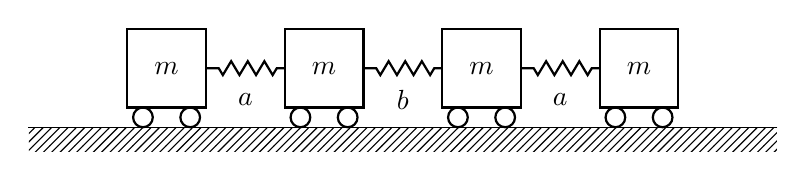
\begin{tikzpicture}
\tikzstyle{spring}=[thick,decorate,decoration={zigzag,pre length=0.1cm,post length=0.1cm,segment length=6}]

\tikzstyle{ground}=[fill,pattern=north east lines,draw=none,minimum width=0.75cm,minimum height=0.3cm]

\node (M) [draw,outer sep=0pt,thick,minimum width=1cm, minimum height=1cm] {$m$};
\node (M2) [draw,outer sep=0pt,thick,minimum width=1cm, minimum height=1cm] at (2,0) {$m$};
\node (M3) [draw,outer sep=0pt,thick,minimum width=1cm, minimum height=1cm] at (4,0) {$m$};
\node (M4) [draw,outer sep=0pt,thick,minimum width=1cm, minimum height=1cm] at (6,0) {$m$};

\node (ground) [ground,anchor=north,xshift=3cm,yshift=-0.25cm,minimum width=9.5cm] at (M.south) {};

\draw (ground.north east) -- (ground.north west);
\draw [thick] (M.south west) ++ (0.2cm,-0.125cm) circle (0.125cm)  (M.south east) ++ (-0.2cm,-0.125cm) circle (0.125cm);
\draw [thick] (M2.south west) ++ (0.2cm,-0.125cm) circle (0.125cm)  (M2.south east) ++ (-0.2cm,-0.125cm) circle (0.125cm);
\draw [thick] (M3.south west) ++ (0.2cm,-0.125cm) circle (0.125cm)  (M3.south east) ++ (-0.2cm,-0.125cm) circle (0.125cm);
\draw [thick] (M4.south west) ++ (0.2cm,-0.125cm) circle (0.125cm)  (M4.south east) ++ (-0.2cm,-0.125cm) circle (0.125cm);

\draw [spring] (M2.180) -- ($(M.north east)!(M.180)!(M.south east)$);
\draw [spring] (M3.180) -- ($(M2.north east)!(M2.180)!(M2.south east)$);
\draw [spring] (M4.180) -- ($(M3.north east)!(M3.180)!(M3.south east)$);

\node at (1,-0.4) {$a$};
\node at (3,-0.4) {$b$};
\node at (5,-0.4) {$a$};

\end{tikzpicture}
\end{center}
\caption{The spring system for $n=4$ masses}
\end{figure}

Setting up the general differential equation, assuming no friction, we get
\[
m\frac{d^2}{dt^2} \mathbf{\hat{x}} + \mathbf{K \hat{x}} = 0
\]
where $\mathbf{\hat{x}}$ is a vector containing the relative positions of each mass, $\mathbf{K}$ is the compression matrix shown below if $n$ is even:
\[
\begin{pmatrix}
a & -a &  &  & \dots & 0\\
-a & a+b & -b &  & \dots & \\
 & -b & a+b & -a & \dots & \vdots \\
 &  & -a & a + b & \dots & \\
\vdots &  &  &  & \ddots & \\
0 &  &  & \dots & -a & a
\end{pmatrix}
\]
and if $n$ is odd:
\[
\begin{pmatrix}
a & -a &  &  & \dots & 0\\
-a & a+b & -b &  & \dots & \\
 & -b & a+b & -a & \dots & \vdots \\
 &  & -a & a + b & \dots & \\
\vdots &  &  &  & \ddots & \\
0 &  &  & \dots & -b & b
\end{pmatrix}
\]

Solving for the eigenvalues of $\mathbf{K}$ symbolically using the following sympy code for the case $n=8$ masses:


\begin{lstlisting}[language=Python]
from sympy import *

a, b = symbols("a b'")

def generateMatrix(li):
    mat = []
    li.append('q')
    for i,x in enumerate(li):
        if i is 0:
            mat.append([x, - x, *[0]*(len(li)-2)])
        elif i is (len(li) - 1):
            mat.append([*[0]*(len(li)-2),- li[-1],li[-1]])
        else:
            last = li[i - 1]
            mat.append([*[0]*(i-1), - last, last + x, - x, \
            *[0]*(len(li) - 2 - i)])
    return Matrix(mat)

sevenSpring = [a,b,a,b,a,b,a]
eightMasses = generateMatrix(sevenSpring)
eightEigen = eightMasses.eigenvals()
pprint(simplify(eightEigen))
\end{lstlisting}

From running the above code on cases for $n=4,6,8,10,12$, we determined that the eigenvalues follow the following order: First, there will always be two "trivial" eigenvalues that follow for all even $n$:
\[
\lambda = 0,  2a
\]
For cases $n>2$, there are the following additional eigenvalues:
\[
\lambda = a + b \pm \sqrt{a^2 + b^2 \pm \lambda' a b}
\]

Where $\lambda'$ was an undetermined variable. Using the code above, we determined the following values of $\lambda'$ for the following values $n$:

\begin{center}
	\begin{tabular}{ c | c}
		$n$ & $\lambda'$ \\
		\hline
		$4$ & $0$ \\
		$6$ & $\pm 1$\\
		$8$ & $0$, $\pm \sqrt{2}$\\
		$10$ & $\frac{\pm 1 \pm \sqrt{5}}{2}$\\
		$12$ & $0$, $\pm 1$, $\pm \sqrt{3}$
	\end{tabular}
\end{center}

It is thus my conjecture that $\lambda'$ is actually:
\[
\pm \lambda' = -2\cos\theta
\]
which allows us to build the following relation:
\begin{center}
	\begin{tabular}{ c | c | c}
		$n$ & $\lambda'$  & $\theta$\\
		\hline
		$4$ & $0$  & $\frac{\pi}{2}$\\
		$6$ & $\pm 1$ & $\frac{\pi}{3}, \frac{2 \pi}{3}$ \\
		$8$ & $0$, $\pm \sqrt{2}$ & $\frac{\pi}{4}, \frac{\pi}{2}, \frac{3\pi}{4}$\\
		$10$ & $\frac{\pm 1 \pm \sqrt{5}}{2}$ & $\frac{\pi}{5}, \frac{2\pi}{5}, \frac{3\pi}{5},\frac{4\pi}{5}$\\
		$12$ & $0$, $\pm 1$, $\pm \sqrt{3}$ &$\frac{\pi}{6}, \frac{\pi}{3}, \frac{\pi}{2}, \frac{2\pi}{3}, \frac{5\pi}{6}$\\
		$\vdots$ & $\vdots$ & $\vdots$\\
		$2k$ & $-2\cos(a_j)$ & $a_j = \frac{j \pi}{k}$ ; $j \in 0<\mathbb{N} < k$
	\end{tabular}
\end{center}

This allows us to generalize the eigenvalues into:
\[
\lambda = a + b \pm \sqrt{a^2 + b^2 - 2 a b \cos(\theta)}
\]
for the $\theta$s given above. It is thus easy to represent this visually as vectors, assuming that $a > b$, $a \dot b = a b \cos(\theta)$ with $c$ being the hypotenuse of both these legs:
\begin{figure}[H]
\begin{center}
\begin{tikzpicture}[scale=3]
% place coordinates at the two initial vertices 
\coordinate (a) at (-2,0);
\coordinate (b) at (0,0);

% automatically calculate the third vertex
\path[name path=line 1] (0,0) -- (120:0.85);
\path[name path=line 2] (-2,0) -- (120:0.85);
\path [name intersections={of=line 1 and line 2, by={c}}];
%\path[name path = line 3] (2,0) -- 

% draw the lines
\draw[dashed] (a) -- (c); %hypotenuse
\draw (a) -- (b); %adjacent
\draw (b) -- (c); %opposite

\node at (-1,-0.15) {$a$};
\node at (-0.1, 0.5) {$b$};
\node at (-1.2, .6) {$c$};

% draw the arc clipping a circle against the triangle and place the label
\path[clip] (a) -- (b) -- (c) -- cycle;
\node[circle,draw,minimum size=80pt] at (0,0) (circ) {};
\node[minimum size = 30pt, left] at (circ.140) {$\frac{\pi}{3}$};
\end{tikzpicture}
\end{center}
\caption{eigenvalue for $n=6$ and $\theta = \frac{\pi}{3}$}
\end{figure}

\begin{figure}[H]
\begin{center}
\begin{tikzpicture}[scale=3]
% place coordinates at the two initial vertices 
\coordinate (a) at (-2,0);
\coordinate (b) at (0,0);

% automatically calculate the third vertex
\path[name path=line 1] (0,0) -- (30:0.85);
\path[name path=line 2] (-2,0) -- (30:0.85);
\path [name intersections={of=line 1 and line 2, by={c}}];

% draw the lines
\draw[dashed] (a) -- (c); %hypotenuse
\draw (a) -- (b); %adjacent
\draw (b) -- (c); %opposite

\node at (-1,-0.15) {$a$};
\node at (0.5, 0.15) {$b$};
\node at (-.5, .4) {$c$};

% draw the arc clipping a circle against the triangle and place the label
\path[clip] (a) -- (b) -- (c) -- cycle;
\node[circle,draw,minimum size=20pt] at (0,0) (circ) {};
\node[minimum size = 40pt, left] at (circ.60) {$\frac{2\pi}{3}$};
\end{tikzpicture}
\end{center}
\caption{eigenvalue for $n=6$ and  $\theta = \frac{2\pi}{3}$}
\end{figure}

For odd $n$, the scheme is similar but has some peculiarities. To illustrate these peculiarities, I will compare the cases for $n$ is odd and $n$ is even:

\begin{center}
	\begin{tabular}{ c | c || c | c}
		$n$  & $\theta_n$ & $2n$ & $\theta_{2n}$\\
		\hline
		$3$ & $\frac{\pi}{3}$ & $6$ & $\frac{\pi}{3}, \frac{2 \pi}{3}$ \\
		$5$ & $\frac{\pi}{5}, \frac{3\pi}{5}$ & $10$ & $\frac{\pi}{5}, \frac{2\pi}{5}, \frac{3\pi}{5},\frac{4\pi}{5}$\\
		$7$ & $\frac{\pi}{7}, \frac{3\pi}{7},\frac{5\pi}{7}$ & $14$ &$\frac{\pi}{7}, \frac{2\pi}{7}, \frac{3\pi}{7}, \frac{4\pi}{7}, \frac{5\pi}{7}, \frac{6\pi}{7}$\\
		$\vdots$ & $\vdots$ & $\vdots$ & $\vdots$\\
		$k$ & $a_j = \frac{(2j-1)\pi}{k}$; $j \in 0<\mathbb{N} < k$ & $2k$ & $a_j = \frac{j \pi}{k}$ ; $j \in 0<\mathbb{N} < k$
	\end{tabular}
\end{center}

Additionally,the "trivial" eigenvalue of $2a$ is no longer an eigenvalue of $\mathbf{K}$ when $n$ is odd, but $0$ remains an eigenvalue. This makes sense, as the $0$ eigenvalue for the free ends represents uniform translation of all masses in the system. Additionally, this means that swapping the values of $a$ and $b$ will have no change whatsoever on systems with odd $n$, while the only change on systems with even $n$ will be trivial eigenvalue $2a$ being replaced with $2b$. 

\end{document}
